\chapter{Results}

\section{Hardware}
The hardware used to produce the results is the Samsung Nexus S (cobranded with
Google) running Android 2.3.4. The official specifications of the device can be
obtained from the manufacturer's website [link to website with reference] A
short listing of the sensors present on the device is given below based on how
the device reports the sensors via the software APIs:

\begin{enumerate}
\item KR3DM 3-axis Accelerometer
\item AK8973 3-axis Magnetic field sensor
\item AK8973 Orientation sensor
\item GP2A Light sensor
\item GP2A Proximity sensor
\item K3G Gyroscope sensor
\item Gravity Sensor
\item Linear Acceleration Sensor
\item Rotation Vector Sensor
\end{enumerate}

It may be noted that of these sensors, the Gravity sensor, the Linear
Acceleration Sensor and the Rotation Vector Sensor are derived sensors. They
depend on filtering the raw data sensed via the accelerometer and the
magnetometer to generate their sensed values. In essence, the Gravity sensor is
a low pass filter over the accelerometer values (since gravity is essentially
stable for the device at a particular orientation), the Linear Acceleration
Sensor is a high pass filter over the accelerometer values (the high frequency
changes in acceleration are presumed to occur due to device motion and thus
correspond to linear acceleration of the device) and the Rotation Vector Sensor
is a composite sensor that fuses Gravity information derived from the
3 axis Accelerometer and the magnetic field information derived from the
3 axis Magnetic field sensor to orient the device in the 3 Dimensional World 
Coordinate space. The actual method used to do so is described in the API
documentation \todo{Provide Reference}[reference to API documentation] and
further discussion is out of scope for this thesis.

\begin{figure}
\centering
    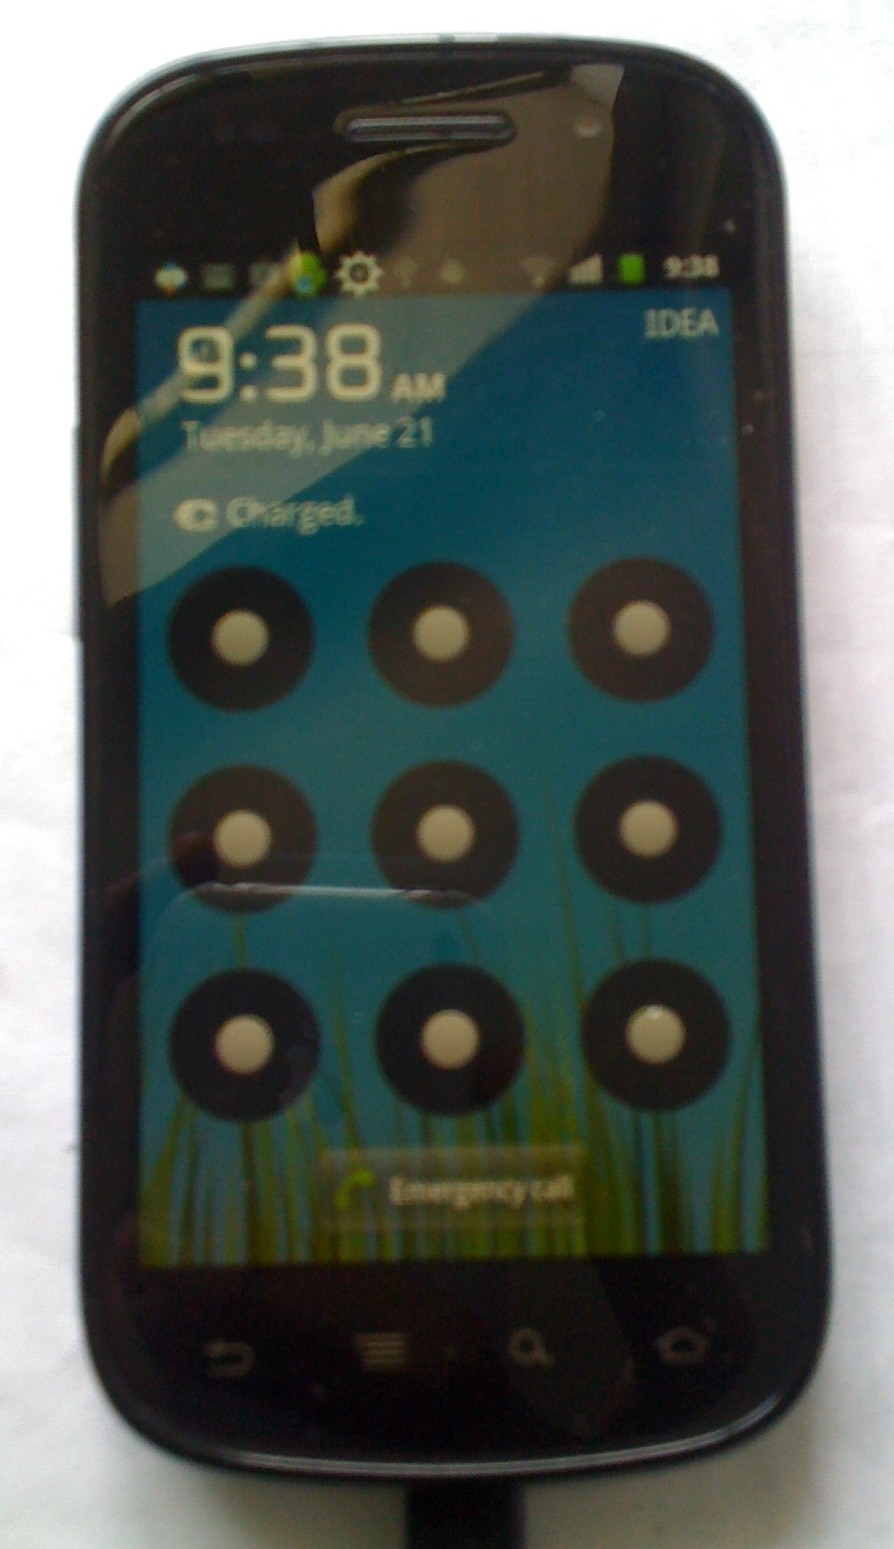
\includegraphics[height=3in]{figures/android_front}
    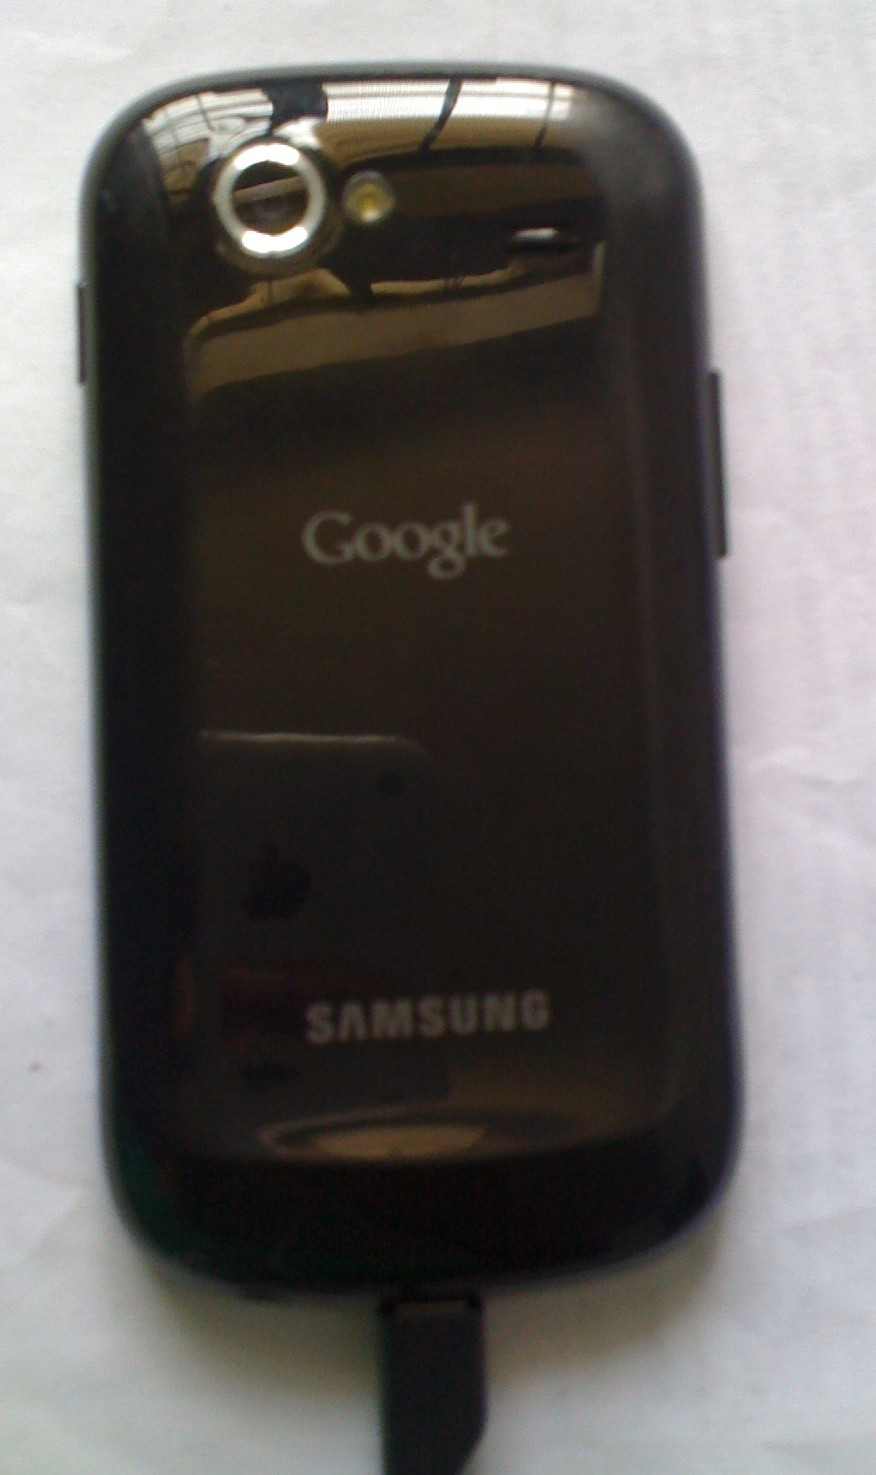
\includegraphics[height=3in]{figures/android_back}
\caption{Google Nexus S manufactured by Samsung}
\end{figure}

\section{Location Under Test}

The location chosen for performing all experimental verification of the
proposed work was Floor 3, Wing 6 and 7 of Ravindra Bhawan at the IIT Roorkee
campus. The environment is suitable for this purpose due to a number of reasons:

\begin{enumerate}
\item There are a large number of Wifi Access Points in close proximity 
    installed on the premises.
\item Wifi Access Points of neighbouring wings and floors provide diversity
    to the location fingerprints.
\item Long corridoors of around 30-32 metres each provide long stretches of
    similar environment for evaluation of algorithm performance over larger
    distances.
\end{enumerate}

A map of the location is shown in Figure \ref{fig:ravindra_map}. The red lines
indicate walls, blue lines indicate windows and green lines indicate doors.
Wifi Access Points are marked with stars on the map. This map has been used
for all the experiments detailed below.

\begin{figure}
    \centering
    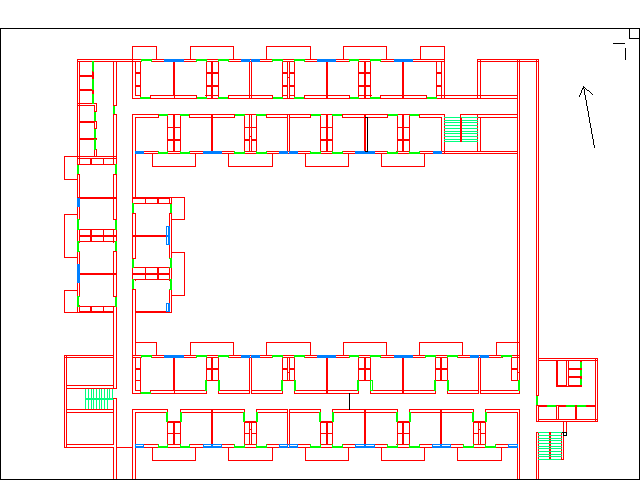
\includegraphics[width=5in]{figures/ravindra_map.png}
    \caption{A map of the experimental environment\label{fig:ravindra_map}}
\end{figure}



\section{Step detection procedure}

Step detection for dead reckoning was done using accelerometer sensor data.
Two different methods were employed and the simple zero crossing method on 
unfiltered data was used as control to estimate the increase in accuracy of the
step detection procedure. A simple clamping technique was employed to filter the
raw acceleration as described in Section \ref{sec:NoiseClamping}.

The effect of the clamping on the raw accelerometer data is shown in 
Figure \ref{fig:accel_raw}. Figure \ref{fig:accel_diff} shows the sensor noise
that is rejected around zero enabling clean detection of peaks corresponding to
the steps.

The comparative graph of the performance of the step detection procedures 
is shown in Figure \ref{fig:csteps}. The correspondence to the ground truth
is shown in Table \ref{tbl:step_table}.

\begin{table}[tbph]
\centering
\begin{tabular}{||l|c||}
\hline
\hline
\textbf{Algorithm} & \textbf{Steps Detected} \\
\hline

Simple Zero Crossings Count & 109 \\
Zero Crossings on Filtered Data & 41 \\
Peaks and Valley Method & 41 \\
\textbf{Ground Truth} & \textbf{40} \\
\hline
\hline
\end{tabular}
\caption{Step Detection Performance\label{tbl:step_table}}
\end{table}

It can be seen that a simple Zero Crossing method performs similarly to the 
Peaks and Valley method. From the time based graph plotted in 
Figure \ref{fig:csteps}, it can be seen that the Peaks and Valley method 
slightly lags the Zero Crossing method in time. This is to be expected as this
method detects a step only when the next peak is detected and thus suffers a 
lag of about half a step.

\begin{figure}[tbph]
    \centering
    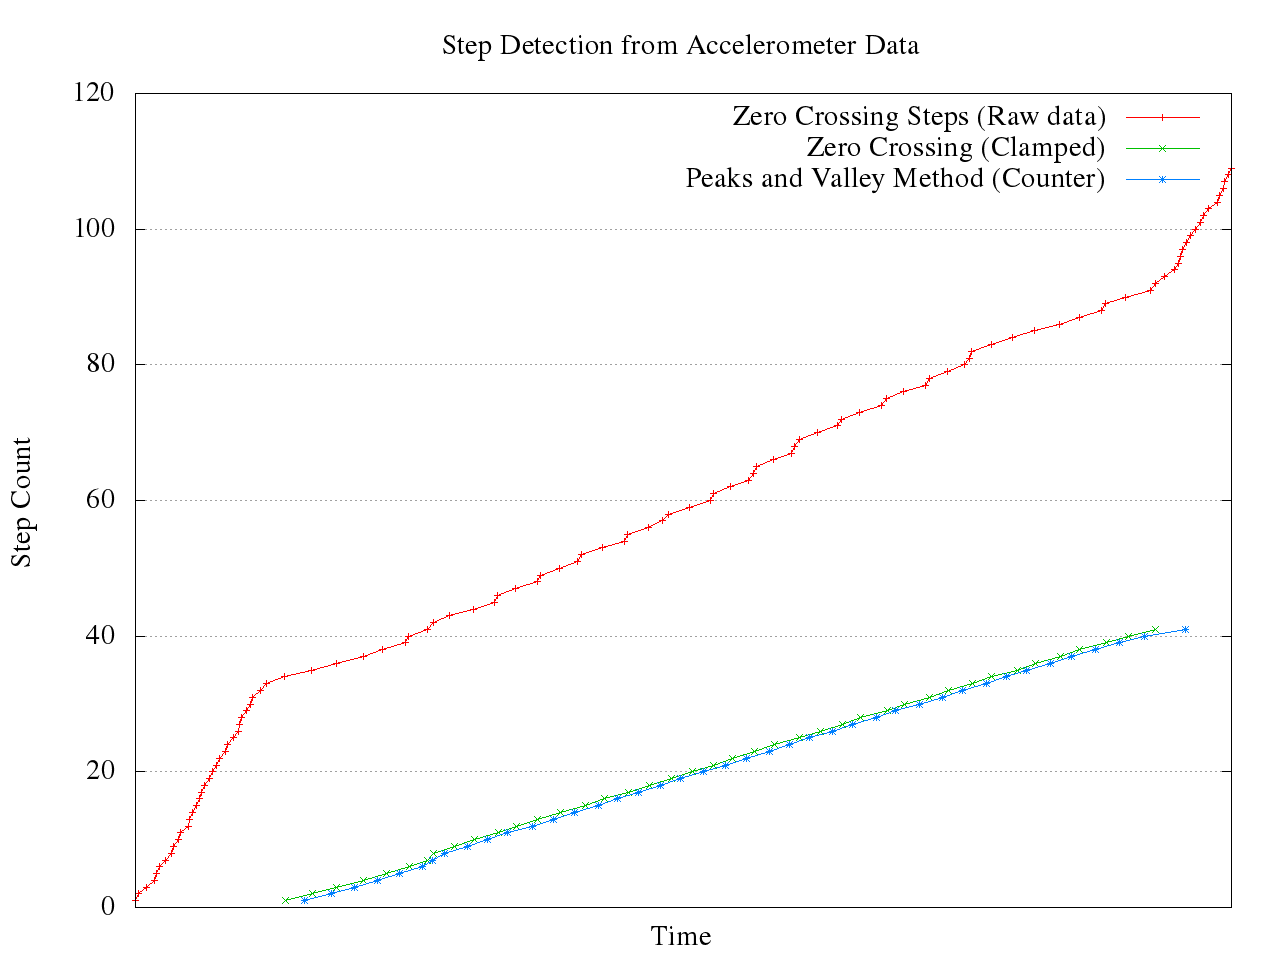
\includegraphics{figures/csteps.png}
    \caption{Performance of Step Detection Algorithms\label{fig:csteps}}
\end{figure}

\begin{figure}[tbph]
    \centering
    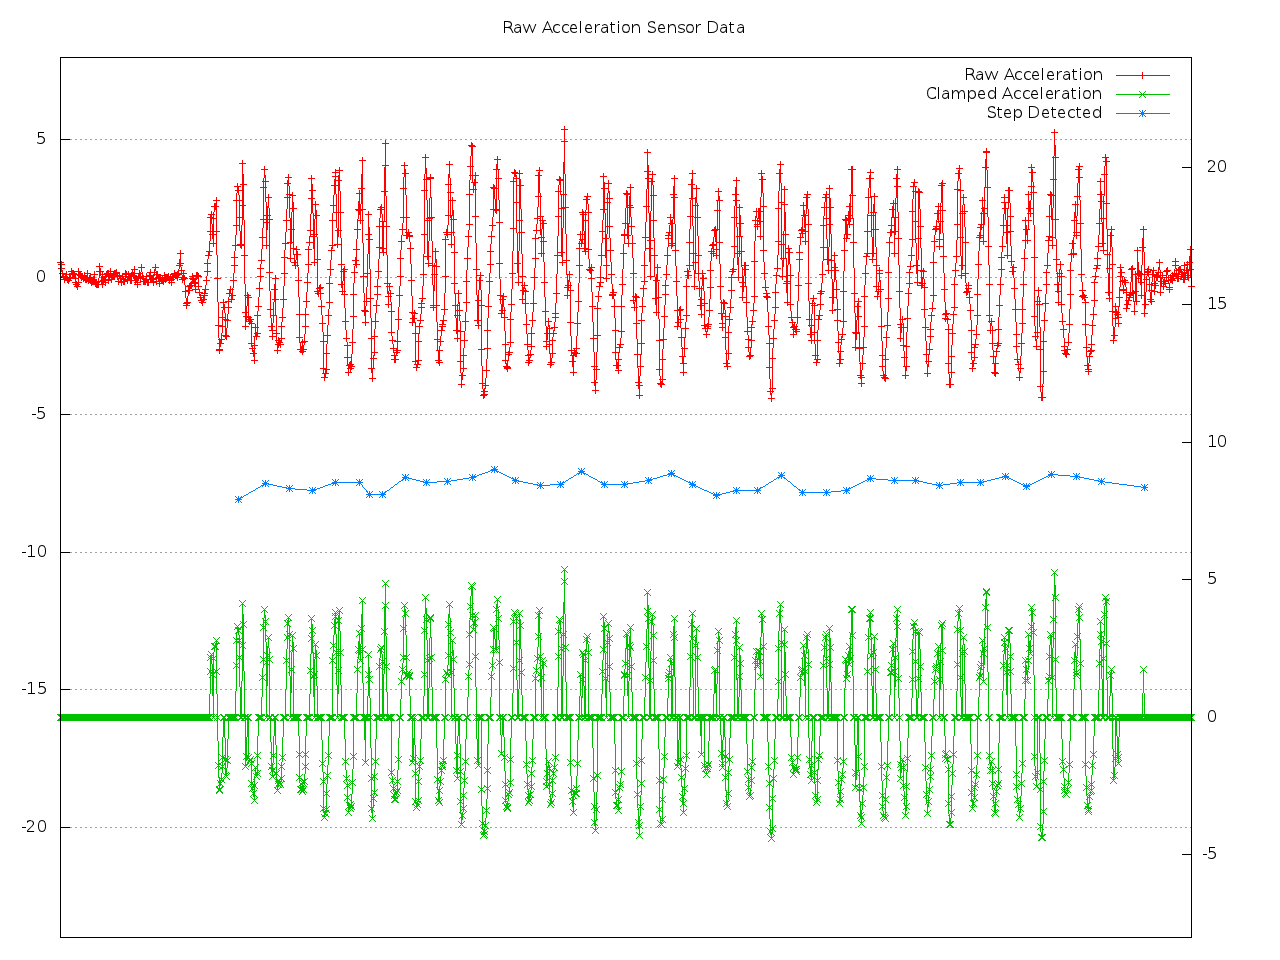
\includegraphics{figures/accel_raw.png}
    \caption{Performance of the Filtering algorithm \label{fig:accel_raw}}
\end{figure}

\begin{figure}[tbph]
    \centering
    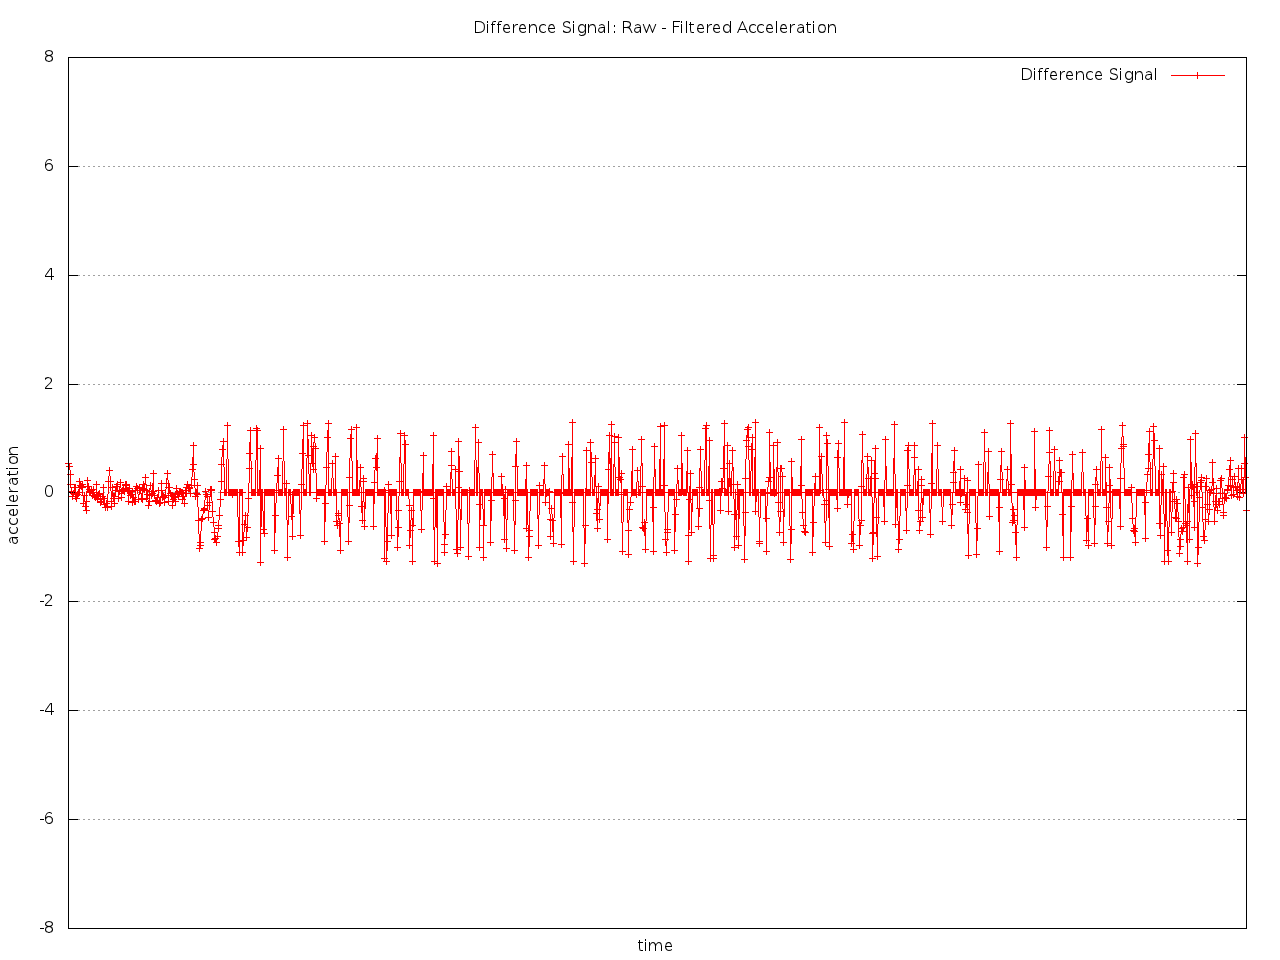
\includegraphics{figures/accel_diff.png}
    \caption{Rejected signal from the Accelerometer sensor \label{fig:accel_diff}}
\end{figure}


\section{First Fix}

For any dead reckoning algorithm, it is important to provide a good starting
point. Low error in the starting location contributes to better
tracking performance.

In order to provide the starting point to the algorithm two approaches were
implemented:

\begin{enumerate}
\item Directly choose the starting location on a map using the capacitive 
    touchscreen
\item Select the starting location based on QRCode recognition using the onboard
    camera. The QRCodes were printed and pasted at specific locations 
    in the area under test.
\end{enumerate}

\missingfigure{QRCodes pasted on the wall}

\subsection{Experimental setup}

All the experments were performed with the same Android device (the Samsung 
Nexus S) and with the same application software. Users were familiar with 
touch screen phones and were well aware of the layout of the building. None of
the users had had any prior exposure to the map of the building and did not 
know the direction of True North. Details of the experiments performed 
are specified in Sections \ref{sec:direct_selection} and \ref{sec:qrcode_selection}

\subsection{Direct Selection of Location on a Map\label{sec:direct_selection}}

Five test subjects were asked to mark out their current position on a
map by simply touching the corresponding location on the map shown on the 
touchscreen of the device. The map was shown at a fixed resolution to all 
test subjects in order to make their responses comparable. 

The test were also allowed to retry locating themselves on the map in case they
were not satisfied with their initial results. All their location attempts were
logged for later analysis.The following facts were observed during the process of 
selection:

\begin{enumerate}
\item Users had an initial difficulty in orienting themselves with regard to 
    the map supplied.
\item As the map contained blocks of rooms that were similar looking, users
    made initial errors in orienting themselves. However, they attempted to 
    correct their errors when the mistake was realized.
\item Some users felt extremely frustrated by the direct selection procedure
    primarily because they could not mark out their locations precisely due
    to the large surface area of contact of their fingers with the touch
    screen. The variability of selection of the contact point while using 
    the touchscreen contributed to an increase in the number of attempts
    required to correctly mark their positions on the map.
\end{enumerate}

%\todo[inline]{Ask 5 people to select locations on a map and log data}
%\missingfigure{Table of error from true location}
%\missingfigure{Table of number of times attempted for satisfactory positioning}

\subsection{Camera based QRCode Method \label{sec:qrcode_selection}}

To evaluate the efficiency of determining first fix via QRCodes in comparison 
to the direct location selection method, an experiment was set up. 
The experiment was performed in conjunction with the experment of 
Section \ref{sec:direct_selection}, users were asked to locate themselves
by snapping a QRCode pasted on the wall instead of marking their starting 
location on a map.

The users were then positioned at various distances from the QRCode and 
asked whether they would make the effort to go to the QRCode to snap their
starting location while using the application or whether they would prefer
the manual method.

The following observations were made regarding the QRCode method for first
fix:

\begin{enumerate}
\item QRCode selection via the camera was a fast process, usually not requiring
    more than 10 seconds on behalf of the user.
\item Users were consistently located at distances less than 1 meter from 
    the QRCode. In most cases, the users were at a distance of around 30 cm 
    from the QRCode pasted on the wall. 
\item There was an instance where poor lighting delayed the capture of the
    QRCode and the QRCode could be successfully captured only after a 
    fluorescent tubelight was switched on to provide adequate lighting.
\end{enumerate}

\missingfigure{Image of a person snapping the QRCode with the camera}

\subsection{Comparison between the two methods}

After processing the results of the experiments, it was determined that 
users overwhelmingly preferred the QRCode method for first fix acquisition.
They were willing to walk up to $5 m$ to the nearest QRCoded location in 
order to take advantage of the facility.

\todo[inline]{Insert survey results}

\subsection{User Feedback}

Users in their comments indicated that potential improvements to the 
application were possible. For example, if the application could determine 
roughly their current location and then provide just that subset of the map
in which the user was located, the speed of providing the first fix location 
by a manual method could be improved.

\section{Determining the Training Constant}

In a separate experiment, three test subjects were asked to walk between 
2 QRCoded locations. The first fix was taken using the QRCode method and 
the training constant was thus estimated based on the number of steps 
detected and the known distance between the 2 QRCoded locations.

The locations used for this test were along a corridoor and were about $30 m$
apart. The tests were repeated thrice for each subject. The resulting 
step constants were taken as the average of the 3 runs.

\todo[inline]{Determining training constant}
\missingfigure{Table of training constant values}

\section{Step variation analysis}

To see the performance of the algorithm to step variations, an experiment 
was performed wherein a test subject walked at three distinct speeds
along a straight corridoor. The subject paused for a short while between 
the three distinct segments to maintain separation of speeds.

The three segments of the walk had the following
characteristics:

\begin{enumerate}
\item The test subject walked with very light steps, almost shuffling along. 
\item The test subject walked with regular steps along the corridoor.
\item The test subject walked with large steps along the corridoor in a motion
    that approximated running.
\end{enumerate}

The accelerometer graphs and the consequent step detections for this 
experiment are shown in Figure \ref{fig:step_variation}. The tabulated
results of the step detection process are shown in 
Table \ref{tbl:step_variation}. Note that the poor performance for 
shuffling steps is due to acceleration peaks not being sufficiently 
distinguishable from sensor noise and for the fast heavy steps is 
due to generation of spurious peaks while coming to an abrupt halt.
A smooth motion doesn't generate such issues and thus the step 
detection procedure is very accurate for that range.

\begin{table}[tbph]
    \centering
    \begin{tabular}{|l|c|c|}
        \hline
        \hline
        Step Segment & Actual Number of Steps & Steps Detected \\
        \hline
        Light Steps (Shuffle) & 10 & 5 \\
        Regular steps & 10 & 10 \\
        Fast (Heavy) steps & 15 & 18 \\
        \hline
        \hline
    \end{tabular}
    \caption{Step detections under step variations\label{tbl:step_variation}}
\end{table}

\begin{figure}
    \centering
    \includegraphics{figures/step_variation.png}
    \caption{Difference in step sizes and the corresponding variations in 
        step detection and step estimates\label{fig:step_variation}}
\end{figure}

\section{Test Paths\label{sec:test_paths}}

Five different test paths were used to test the performance of the system.
The features of these paths are described below. The paths themselves
are marked out in Figure \ref{fig:test_paths}.

\begin{enumerate}
\item Straight walk down a corridoor (A to B)
\item Straight walk down a corridoor, a U turn followed by a straight walk 
    to the starting point. (A to B and then B to A)
\item Zig-Zag walk down a corridoor (A to B).
\item A U shaped walk along all three corridoors. (A-B-C-D)
\item A U shaped walk along all three corridoors followed by a U turn and a 
    walk back to the starting location. (A-B-C-D-C-B-A)
\end{enumerate}

\begin{figure}
    \centering
    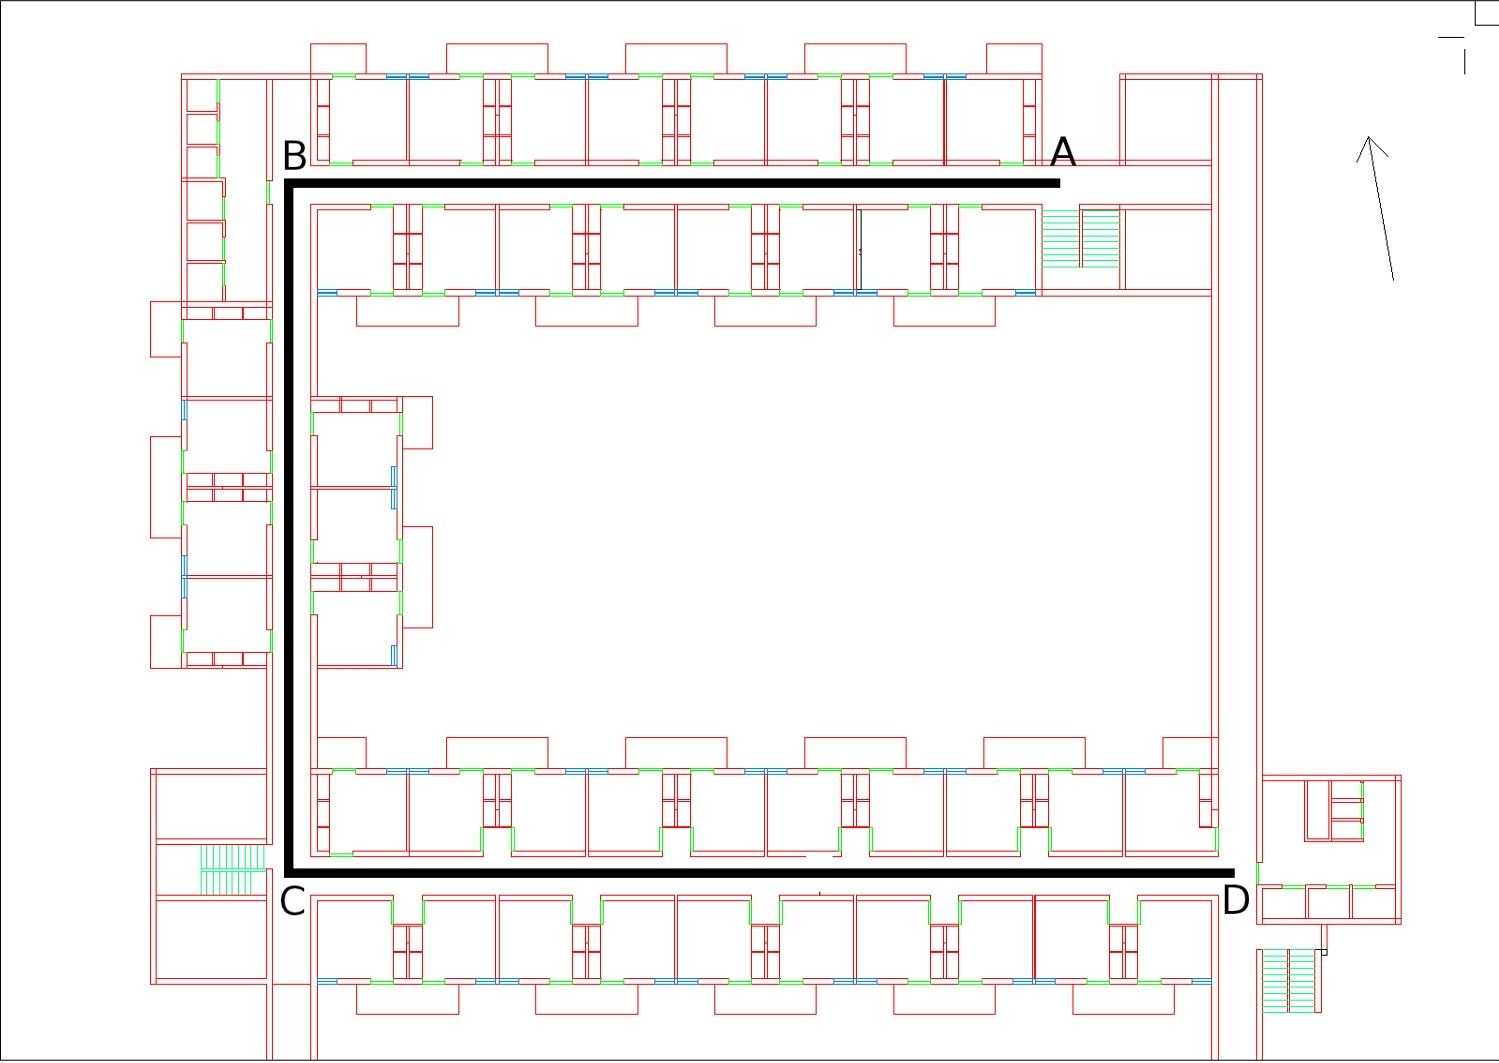
\includegraphics[width=5in]{figures/test_paths.jpg}
    \caption{Test paths for algorithm\label{fig:test_paths}}
\end{figure}


\section{Simple Dead Reckoning}

As discussed in the Literature Review (Chapter \ref{chap:literature_review}) and
in the Proposed Work (Chapter \ref{chap:proposed_method}), it is impossible to
directly obtain displacement information by double integration of the
accelerometer data. Hence, the step detection method was employed for tracking
the motion of the device as held by a walking human. The steps are integrated
with orientation information received from the magnetometer to create a 
simple dead reckoning system in accordance with the dynamical equation 
\eqref{eq:dr_eq}. The initial position for dead reckoning was obtained via
QRCodes in accordance with the description in Section \ref{sec:QRCodes}.


\subsection{Simple Dead Reckoning Results}

One of the well known weaknesses of the dead reckoning approach is that it
diverges quickly from the ground truth unless corrective measures are taken.
As a basic control for the results, a simple dead reckoning based 
tracking algorithm was developed. 

Figure \ref{fig:dr_path1} shows the quick divergence of the algorithm
from the expected path A-B. In fact, at the end of a simple straight walk of 
around $30 m$, the estimate for the location has diverged a lot from the 
actual location. It should also be noted that the path taken passes through
rooms and walls and thus, doesn't look like a natural path for the user.

Figure \ref{fig:dr_path5} shows the extreme divergence that takes place 
over long distances. Table \ref{tbl:dr_error_growth} chronicles the 
error growth that takes place for this path at the turning points of the path.
It is amply clear that Simple Dead Reckoning is not suitable for tracking
if implemented as-is.

\begin{table}[bph]
\centering
\begin{tabular}{l c c}
\hline
\hline
Location    & Distance Travelled    & Error \\
\hline
A           & 0                     & 0 \\
B           & 30 m                  & 3.761 m \\
C           & 56 m                  & 4.982 m \\
D           & 92 m                  & 5.416 m \\
\hline
\end{tabular}
\caption{Error growth over distance for Simple Dead Reckoning\label{tbl:dr_error_growth}}
\end{table}

\begin{figure}
    \centering
    \includegraphics[width=4in]{figures/dr_path1}
    \caption{Performance of Dead Reckoning for Test Path 1\label{fig:dr_path1}}
\end{figure}
 
\begin{figure}
    \centering
    \includegraphics[width=4in]{figures/dr_path5}
    \caption{Performance of Dead Reckoning for Test Path 5\label{fig:dr_path5}}
\end{figure}
 
 

\section{Reckoning with NN Wifi correction}

As per our groundwork described in Section \ref{sec:knn_pos} we know that the 
mean error for positioning using KNN is around $2.8 m$ with a standard deviation
that is nearly the same as the mean. Given the large errors incurred by 
the dead reckoning solution, we wish to analyze the performance of Dead 
Reckoning after Wifi data is integrated into the system.

\subsection{Wifi Survey}

We carried out a Wifi Survey of the test area and collected 1562 samples by 
carefully laying down a $1 m \times 1 m$ grid and collected samples. 8
different samples were collected per grid point at orientations that were
detected to be 45 degrees apart by the onboard magnetometer. By relying on
the magnetometer itself to specify orientation, the effect of local magnetic
fields was taken into account during the survey. However, sensor noise causes
the angle values actually recorded with the Wifi Signal Strength data to vary 
from the expected orientation of the user.

\subsection{Tracking Performance}

While implementing and testing out the implementation of the KNN based 
tracking solution, the resource and scaling limitations of the system 
came to fore. 

Because of it being a ``lazy" algorithm that consults the entire 
training dataset on every query for a position, the KNN algorithm
is computationally very intensive. Queries for obtaining a position based
on Wifi information was a slow process that even disrupted the UI of the 
application due to its heavy workload. Optimizations involving cacheing 
of data and short-circuiting the distance calculation step based on the 
orientation angle of the training sample viz a viz the current device 
orientation were implemented. With these optimizations, we were able 
to successfully run a hybrid Dead Reckoning system that utilized 
Wifi Access Point Received Signal Strengths and Step motion information
to track the device.

The performance of the algorithm was again judged based on the test paths 
mentioned in Section \ref{sec:test_paths}. Figure \ref{fig:nn_path1} shows
the track for Test path 1. A quick glance will indicate that the 
tracked endpoints are reasonably accurate (error < 2m), however, 
the subjective nature of the tracked path is very poor.

\begin{figure}
    \centering
    \includegraphics[width=5in]{figures/nn_path1}
    \caption{Performance of the KNN algorithm for Test Path 1\label{fig:nn_path1}}
\end{figure}

\begin{figure}
    \centering
    \includegraphics[width=5in]{figures/nn_path5}
    \caption{Performance of the KNN algorithm for Test Path 5\label{fig:nn_path5}}
\end{figure}


%\subsection{Case 2: Dead reckoning with KNN averaging}
%\subsection{Case 3: Dead reckoning with clamped wifi positioning}

\section{Reckoning with Integrated Map Information}

The results of the Wifi corrected reckoning as well as the data collected 
as part of the implementation of the KNN positioning system indicates that 
the location information utilizing Wifi data is very unstable. On the other
hand there is significant drift if we depend solely on the accelerometer
and the magnetometer to provide intertial tracking. In order to get 
better accuracy from the system, we require constant feedback from the 
environment. A way to achieve that is to use the fact that the device 
holder is always moving through ``passable" spaces on the map. Any motion
contrary to the allowed locations on the map would indicate tracking drift 
and a feedback loop would be set up to correct for such errors.

In this context, the particle filter's performance is analyzed with the
same test tracks as the other two algorithms. 

As can be seen amply in Figure \ref{fig:pf_path2} and Figure \ref{fig:pf_path4}
the tracking performance of this algorithm is excellent. The drift errors of the 
dead reckoning solution are compensated for by the map information
which ensures that only states consistent with the motion of the device 
are retained. Long term behaviour of the algorithm is also remarkably 
stable. Even after moving close to 100 m, the algorithm was able to 
maintain a tracking error of less than 1 m. This is illustrated in 
Figure \ref{fig:pf_path4}.


\begin{figure}
    \centering
    \includegraphics[width=5in]{figures/pf_path2}
    \caption{Performance of Reckoning with Map information for Test Path 2.\label{fig:pf_path2}}
\end{figure}

\begin{figure}
    \centering
    \includegraphics[width=5in]{figures/pf_path4}
    \caption{Performance of the Reckoning algorithm for Test Path 4.\label{fig:pf_path4}}
\end{figure}

%\subsection{Case 1: Probability of crossing walls is 0}
%\subsection{Case 2: Probability of crossing walls is finite}
%\todo[inline]{Should I even do it? It should come out with poorer results.}

%\subsection{Case 3: Resampling of impoverished data points with duplication}
%\subsection{Case 4: Resampling with introduction of Gaussian noise}
%\subsection{Case 4a: Use of averaged data points v/s random weighted data point}
%\subsection{Case 5: Accounting for bias in orientation sensor}
%\subsection{Case 6: Accounting for step size bias.}
%\subsection{Case 8: Simple heuristics to deal with impoverished samples}
%(retry, retry with greater inaccuracy, wifi)

\section{Comparison with published results}

With additional information at hand as well as suitable modifications to the 
dynamical equations of the system and care in avoiding particle degeneracy,
a significantly better accuracy has been achieved by this system as compared
to previous published works. 

The comparison of the 3 implemented methods can be done via the cumulative
distribution function which maps the percentage of sample points 
expected to be below a given error distance. 

\missingfigure{comparison table between results published and our methods}

\missingfigure{CDF of the errors of the methods (will take some time)}

\section{Summary of Results}
\todo[inline]{Which algorithms to pick based on the results, advantages and disadvantages}

\section{Issues faced}
Incorrect step sizes yielded states in which no further progress was possible
using data from the inertial sensors. Hence we had to resort to wifi data to get
out of the blind spot.

Limited processing power and near-realtime time constraints of operation
constrain computational complexity of the solution.

Surveying is the biggest issue in this system.

Computational complexity and scaling issues.

\begin{figure}
    \centering
    \includegraphics[width=5in]{figures/pf_bad.png}
    \caption{Sometimes, the recovery process leads to a sequence of states 
        which is equivalent to getting lost.\label{fig:pf_bad}}
\end{figure}
